\documentclass[12pt, letterpaper]{article}
\usepackage[utf8]{inputenc}
\usepackage{graphicx}
\usepackage{xspace}
\graphicspath{ {/home/tobiasjenegger/Documents/summary/} }
\title{Radius/Momentum Calculation for S444 Experiment February 2020 - Overview}
\author{Tobias Jenegger}

\begin{document}
\begin{titlepage}
\maketitle
\end{titlepage}
\subsection{The Setup}
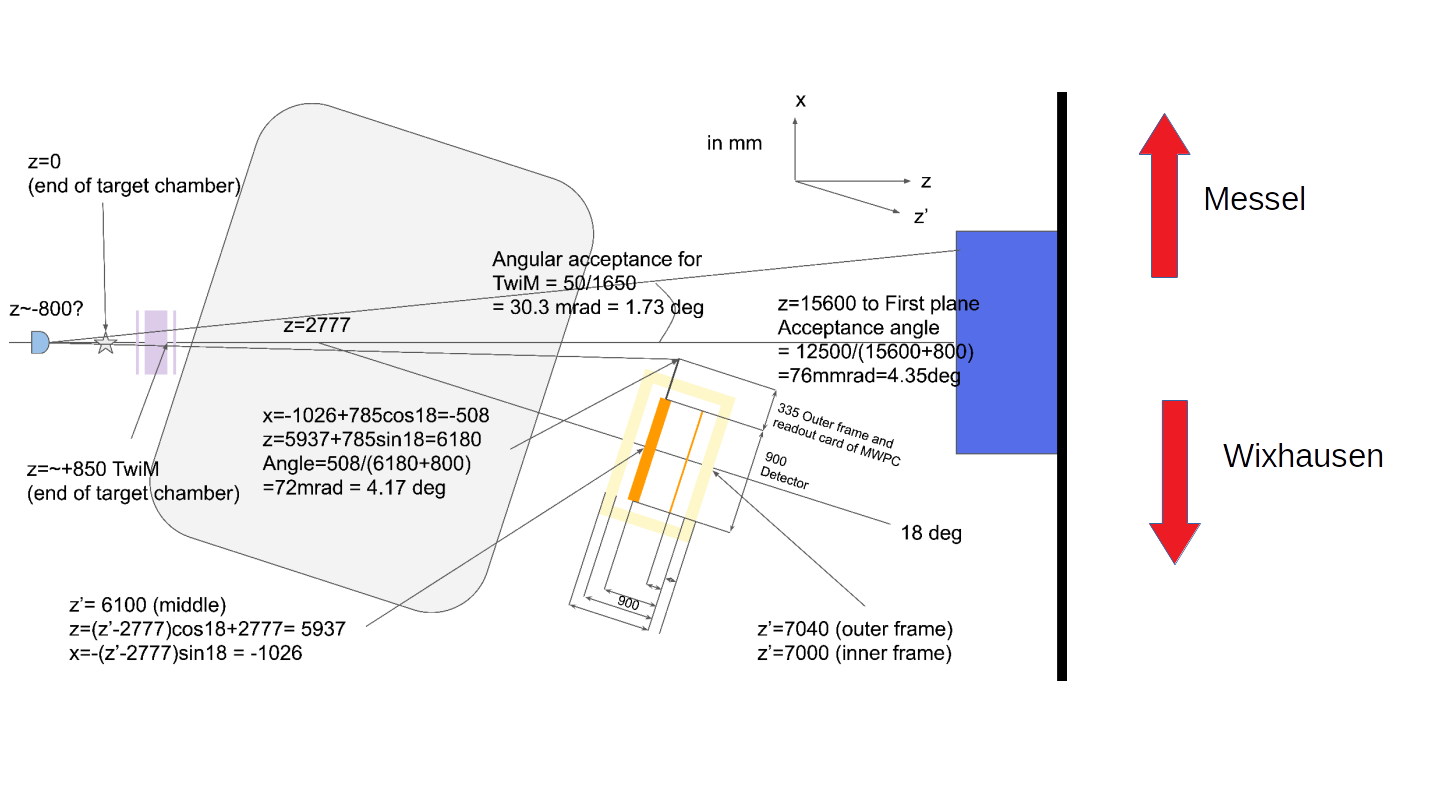
\includegraphics[width=1.2\textwidth]{mes_wixh.png}
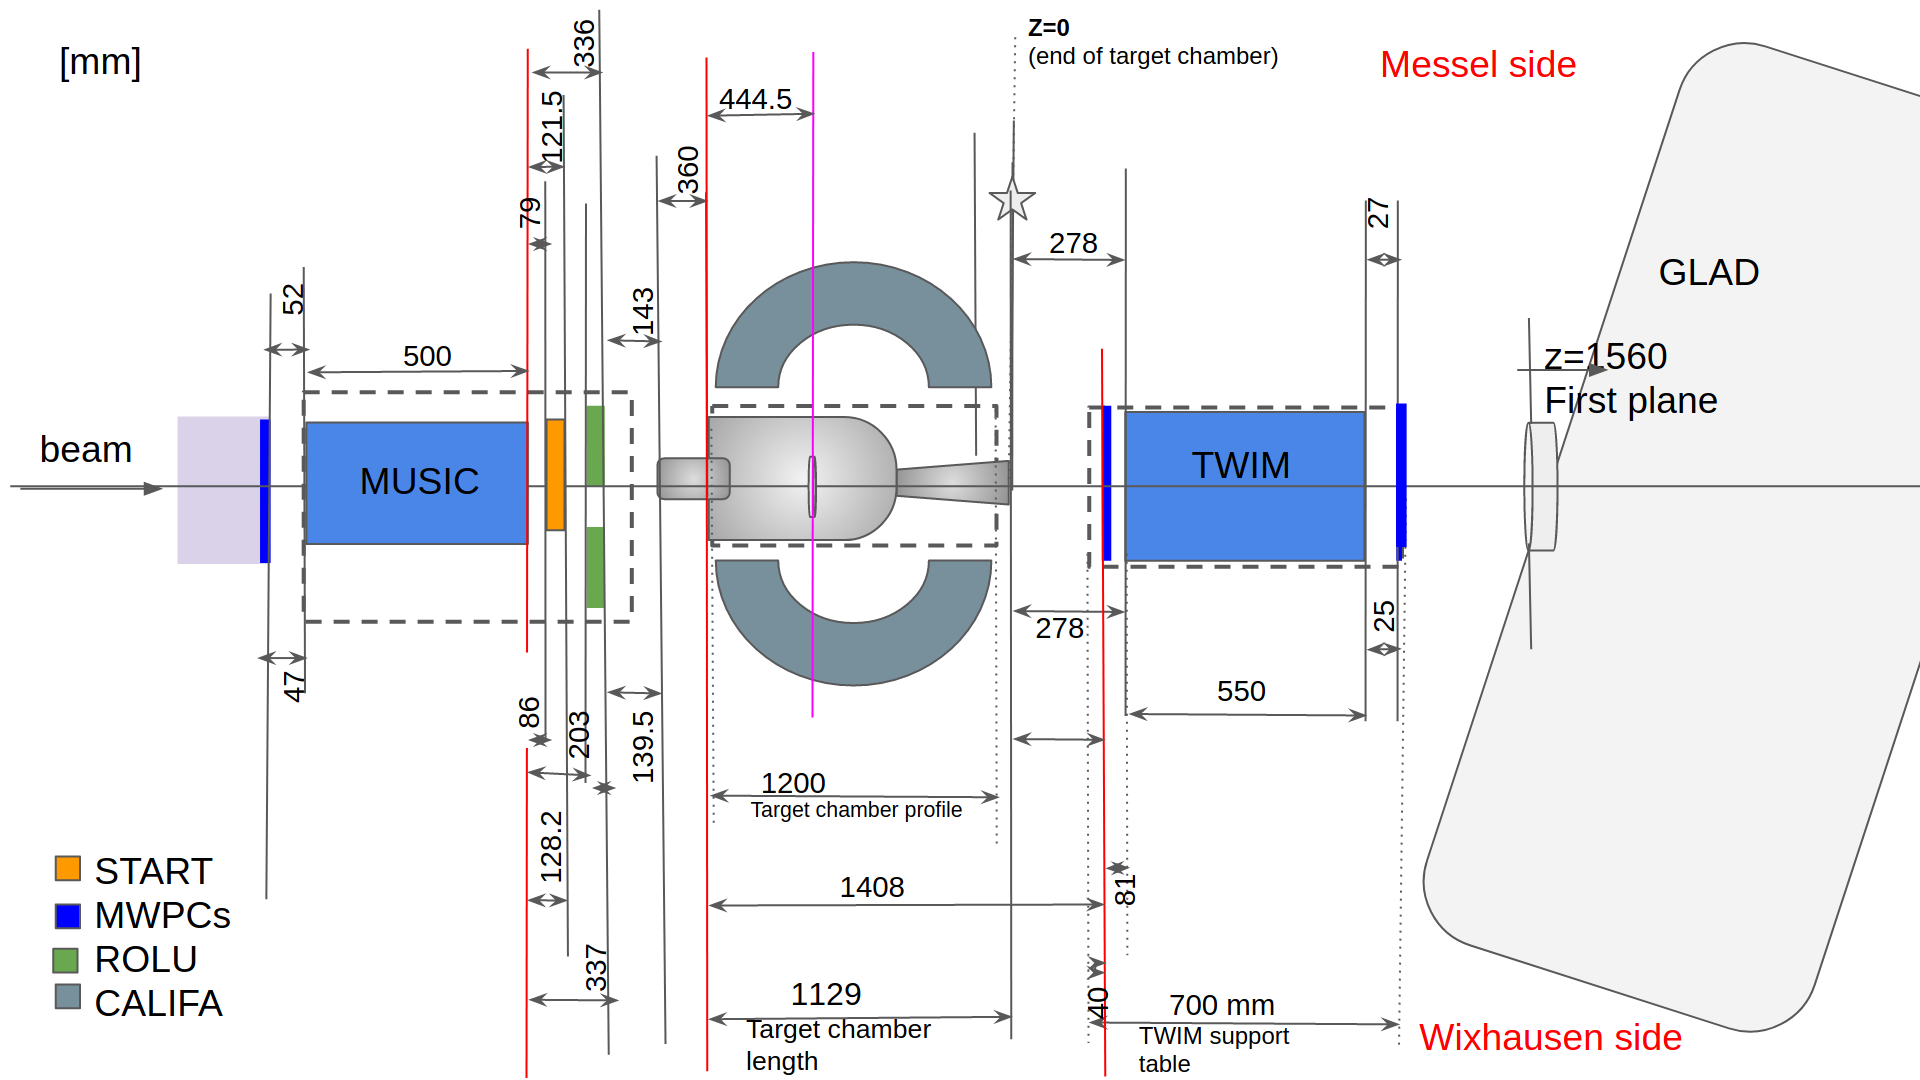
\includegraphics[width=1.2\textwidth]{SETUP_around_Target.png}
\subsubsection{Geometry and relative position of the detectors in the beam direction}
Here, the positions are given for the s444 and s467 experiments\\
z position of the target:    \hspace{10mm} zT = -684.5 mm\\
z position of the MWPC in front of the Twin-MUSIC:  \hspace{10mm}   zM1 = 279 mm \\
z position of the middle of the Twin-MUSIC:  \hspace{10mm}  zTwin = 553 mm\\
z position of the MWPC after the Twin-MUSIC:  \hspace{10mm}   zM2 = 854 mm\\
$\alpha$ tilted angle of GLAD (14 degrees):   \hspace{10mm} = 0.244 rad\\
effective length of GLAD:  \hspace{10mm}   Leff = 2067 mm\\
z middle of GLAD  \hspace{10mm}  zGm = 2577mm\\
horizontal of the central path (18 degree) \hspace{10mm}   $\theta$\textunderscore out0 = pi/10 rad\\
z position of the MWPC after GLAD   \hspace{10mm}  zM3 = 5937 mm\\
z position of the ToFwall          \hspace{10mm}     zToFW = 6660.2 mm\\

Correspondence between the GLAD current and the magnetic field:  I = 3584 A, B = 2.2 T



\end{document}